\documentclass[../main.tex]{subfiles}

\begin{document}


The following is the definition of the residual.
\begin{center}
    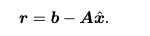
\includegraphics[width=\textwidth,height=\textheight,keepaspectratio]{lec6_resid}
\end{center}

\begin{remark}
    The residual itself does not reveal much. Suppose we calculate $r = b - Ax$. Now solve for $kAx = kb$ and the residual required to solve that is $k$ times as great. This is why we define the relative residual:

    \[
        \frac{\norm{r}}{\norm{A} \cdot \norm{\hat{x}}}
    \]
\end{remark}

We can obtain a bound on the relative forward error required to solve $Ax = b$ in terms of $r$.
\begin{center}
    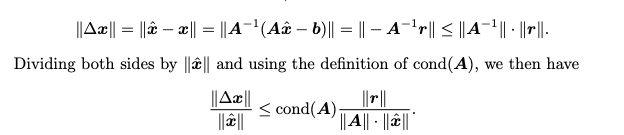
\includegraphics[width=\textwidth,height=\textheight,keepaspectratio]{lec6_residBound}
\end{center}

\begin{remark}
    This bound tells us that if the residual is small and the matrix and well conditioned, then the relative error is low.
\end{remark}

\begin{center}
    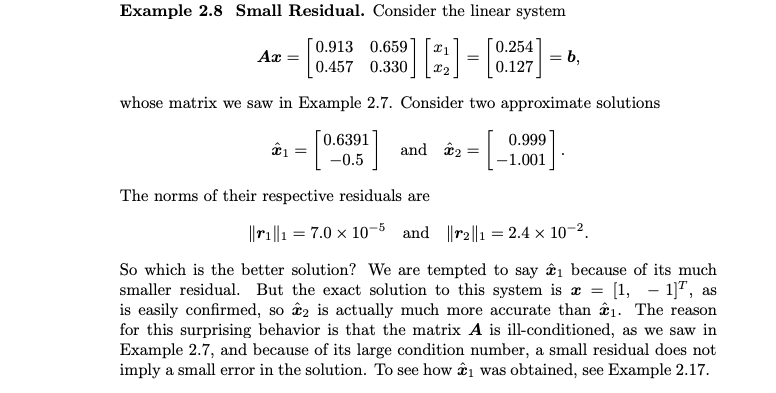
\includegraphics[width=\textwidth,height=\textheight,keepaspectratio]{lec6_residExample}
\end{center}

\begin{center}
    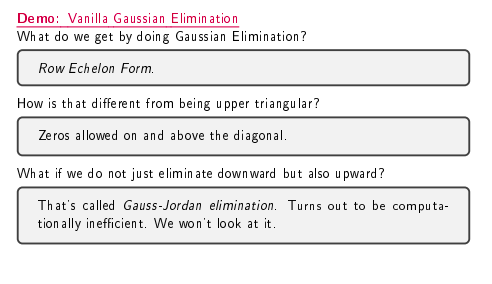
\includegraphics[width=\textwidth,height=\textheight,keepaspectratio]{lec6_rowE}
\end{center}

\begin{remark}
    Also note that a matrix is in row echelon form if the first non-zero entry of each row (what was the pivot during gaussian elimination) is to the first of the first non-zero entry of any preceding row; moreover, entries in rows above the pivot (but in the same column) must be $0$.
\end{remark}

\begin{center}
    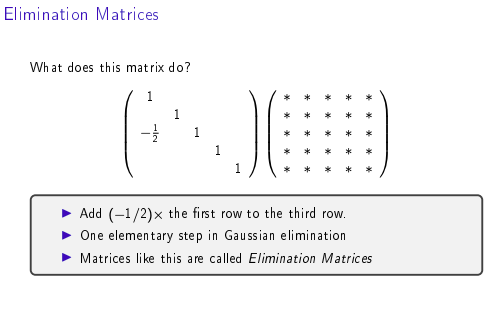
\includegraphics[width=\textwidth,height=\textheight,keepaspectratio]{lec6_elimM}
\end{center}

\begin{remark}
    If we add $k$ to the identity matrix at entry $i,j$, and left multiply the resultant
    matrix $C$ by some matrix of interest $A$, then the result is to take the $j$ th row of $A$
    multiply it by $k$ and then add it to $i$. We can undo this process by using the same
    matrix but, in place of $k$, using $-k$. This second matrix is the inverse to the elimination matrix $C$.
\end{remark}

\begin{center}
    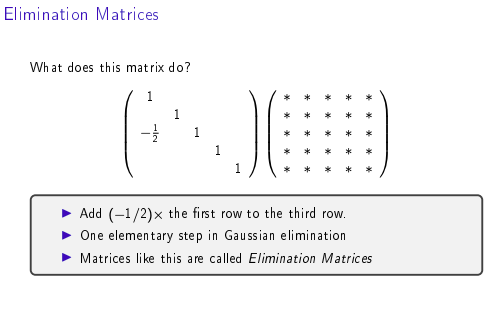
\includegraphics[width=\textwidth,height=\textheight,keepaspectratio]{lec6_elimM}
\end{center}


\begin{remark}
    Suppose that we multiply $A$ by an elimination matrix $M_1$, then by $M_2$ up to $M_l$,
    where $M_l$ is the last matrix required to turn $A$ into Row Echelon Form.
    Eventually, we will have 

    \[
        (M_l \dots M_1)A = U \implies A =  \inv{(M_l \dots M_1)}U
    \]

    At first glance, this is okay, because it turns out that left multiplication of an elimination matrix $X$ by $Y$ such that $X$ has a non-zero off diagonal at column $i$ and $Y$ has a non-zero off diagonal at column $j$ where $i < j$ results in an elimination matrix that just merges $X$ and $Y$ \footnote{Note that merging also takes place if we multiply two elimination matrices that have their off diagonal non-zero entry in the same column as each other.}

    For whatever reason, pivoting foils this attempt:

    \begin{center}
        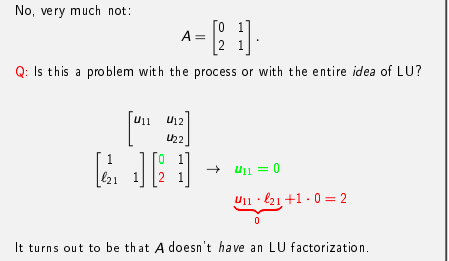
\includegraphics[width=\textwidth,height=\textheight,keepaspectratio]{lec6_pivotfail}
    \end{center}

    The solution is to repeatedly apply permutations to $A$ (in the form
    of permutation matrices) so that the pivot is the largest element
    in terms of absolute value in its column.

    Thus, we now have

    \[
        (M_lP_l \dots M_1P_1)A = U \implies A = \inv{(M_lP_l \dots M_1P_1)}U
    \]

    However, what should be $L$ above is not always left triangular. It can be shown that a factorization of $\inv{(M_lP_l \dots M_1P_1)}$ does, however, give us a lower triangular system.
\begin{center}
    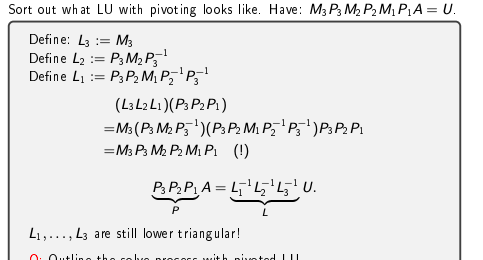
\includegraphics[width=\textwidth,height=\textheight,keepaspectratio]{lec6_pivotres}
\end{center}
\end{remark}

\begin{center}
    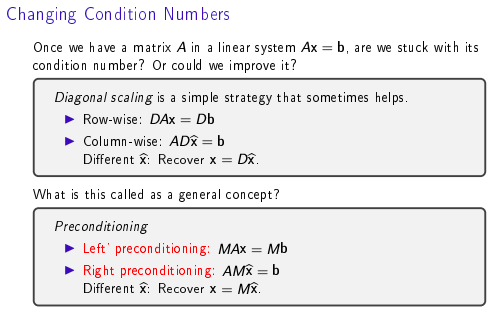
\includegraphics[width=\textwidth,height=\textheight,keepaspectratio]{lec6_precond}
\end{center}
\begin{remark}
    Suppose that $D$ above satisfies $k(D) \approx 1$. Then

    \[
        k(DA) = \norm{DA}\norm{\inv{(DA)}} \leq \norm{D}\norm{A}\norm{\inv{A}}\norm{\inv{D}} \leq k(A)
    \]

    so that the condition number of $K(DA)$ is no greater than the condition number of $A$.

    Assuming that $D$ is invertible, then the set of $x$ satisfying
    $Ax = b$ is precisely the set of $x$ satisfying $Ax = b$. Left multiplication
    by $D$ of $A$ is called, understandably, left preconditioning and scales
    $A$ in a row-wise manner; right multiplication by $D$ of $A$ is called right
    preconditioning.
\end{remark}


\begin{remark}
\begin{center}
    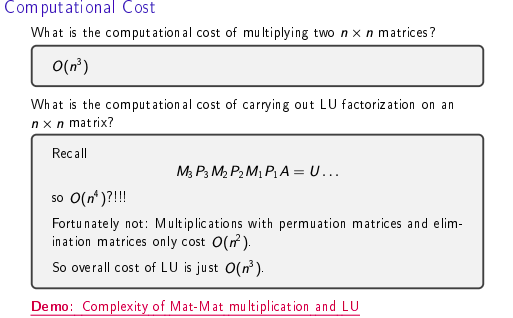
\includegraphics[width=\textwidth,height=\textheight,keepaspectratio]{lec6_compCost}
\end{center}

Multiplication by a permutation matrix is only an $n$ operation, since it involves switching rows. Multiplication by an elimination matrix simply involves scaling one row and mulitplying it by another, and this process is done at most $n$ times for any one elimination matrix (making it $O(n^2)$ as well). Since these transformations are applied at most $n$ times, the process of getting a matrix into $LU$ form is only $O(n^3)$.
\end{remark}

\begin{remark}

\begin{center}
    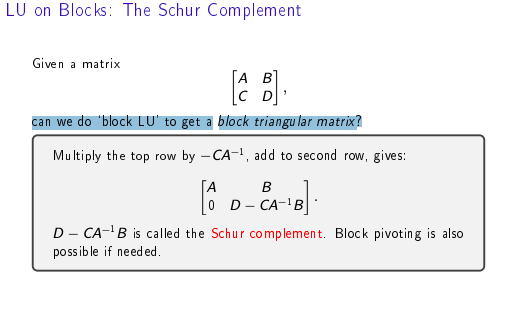
\includegraphics[width=\textwidth,height=\textheight,keepaspectratio]{lec6_luBlocks}
\end{center}

Not sure why this is significant.

\end{remark}


\begin{remark}
    Unresolved
\begin{center}
    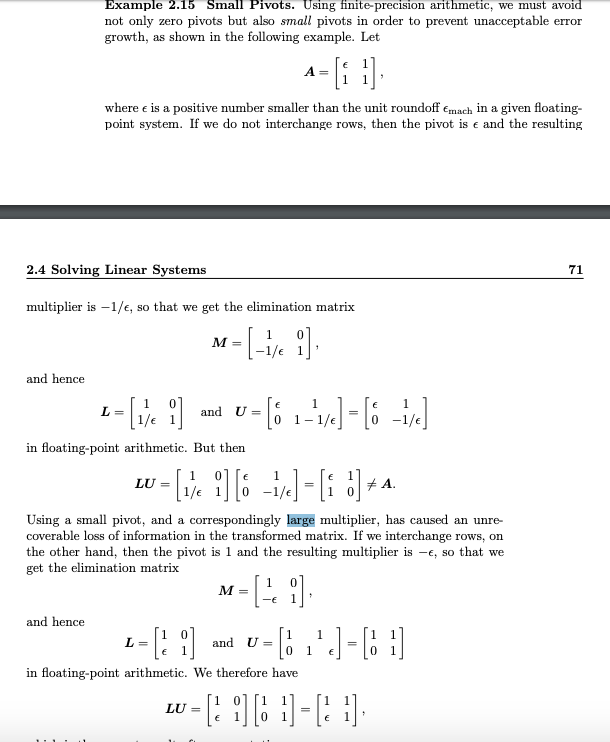
\includegraphics[width=\textwidth,height=\textheight,keepaspectratio]{lec6_smallPivotsBad}
\end{center}
\end{remark}

\begin{remark}
    Notice that if we already have an $LU$ factorization, then computing a rank $1$ update is just an $O(n^2)$ operation.
\begin{center}
    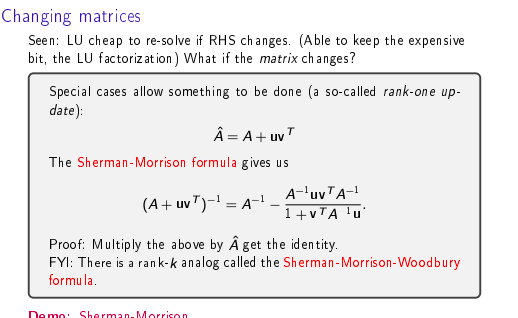
\includegraphics[width=\textwidth,height=\textheight,keepaspectratio]{lec6_shermanMorrison}
\end{center}

For 

\[
    \left( A + uv^T \right)^{-1}b = \inv{A}b - \frac{\left( \inv{A}u \right)v^T\inv{A}b}{1 + v^T\inv{A}u}
\]

And $\inv{A}x$ for any $x$ is an $O(n^2)$ operation. The only other operation in this formula is to compute a dot product.
\end{remark}
\end{document}






\section{Lecture 7}

\subsection{Quiz}




